\section{Korrelationen zwischen Städten und ihrem Umland}
In \autoref{fig:highest_selected_counties} sind die Korrelationswerte zwischen den in  \autoref{sec:selected_counties} beschriebenen Städten und den zugehörigen Landkreisen für eine zeitliche Verschiebung zwischen $\tau=-50$ und $\tau=50$ als Kurven dargestellt.

Die Kurven, deren Maximum rechts der null ist, sind orange eingefärbt. Die Kurven mit dem höchsten Punkt links der null sind blau gefärbt. Die restlichen Kurven, welche am für $\tau=0$ maximal werden, sind grün gefärbt.
Bei den Korrelationsanalysen der folgenden Stadt- (SK) und Landkreise (LK) sind die Werte bei einer Verschiebung $\tau=0$ maximal:
\begin{itemize}
    \item LK Kassel (6633) mit SK Kassel (6611)
    \item LK Südliche Weinstraße (7337) mit SK Landau i.d.Pfalz (7313)
    \item LK Heilbronn (8125) mit SK Heilbronn (8121)
    \item LK Rastatt (8216) mit SK Baden-Baden (8211)
    \item LK Rosenheim (9187) mit SK Rosenheim (9163)
    \item LK Landshut (9274) mit SK Landshut (9261)
    \item LK Straubing-Bogen (9278) mit SK Straubing (9263)
    \item LK Neustadt a.d.Waldnaab (9374) mit SK Weiden i.d.OPf. (9363)
    \item LK Oberallgäu (9780) mit SK Kempten (9763)
\end{itemize}
Bei den Korrelationsanalysen der folgenden Stadt- und Landkreise sind die Werte bei einer Verschiebung $\tau=1$ maximal:
\begin{itemize}
    \item LK Amberg-Sulzbach (9371) mit SK Amberg (9361)
    \item LK Saalekreis (15088) mit SK Halle (15002)
    \item LK Weimarer Land (16071) mit SK Weimar (16055)
\end{itemize}
Bei den Korrelationsanalysen von LK Trier-Saarburg (7235) mit SK Trier (7211) und LK Regensburg (9375) mit SK Regensburg (9362) sind die Werte bei einer Verschiebung $\tau=3$ maximal. Die Werte der Korrelationsanalyse von LK Bamberg (9471) mit SK Bamberg (9461) sind maximal bei einer Verschiebung $\tau=8$.
Die Werte Korrelationsanalysen von LK Südwestpfalz (7340) mit SK Pirmasens (7317), LK Potsdam-Mittelmark (12069) mit SK Brandenburg a.d.Havel (12051) und LK Spree-Neiße (12071) mit SK Cottbus (12052) werden in jeweils bei einer Verschiebung $\tau=-2$, $\tau=-4$ und $\tau=-6$ maximal.
\begin{figure}[H]
    \centering
    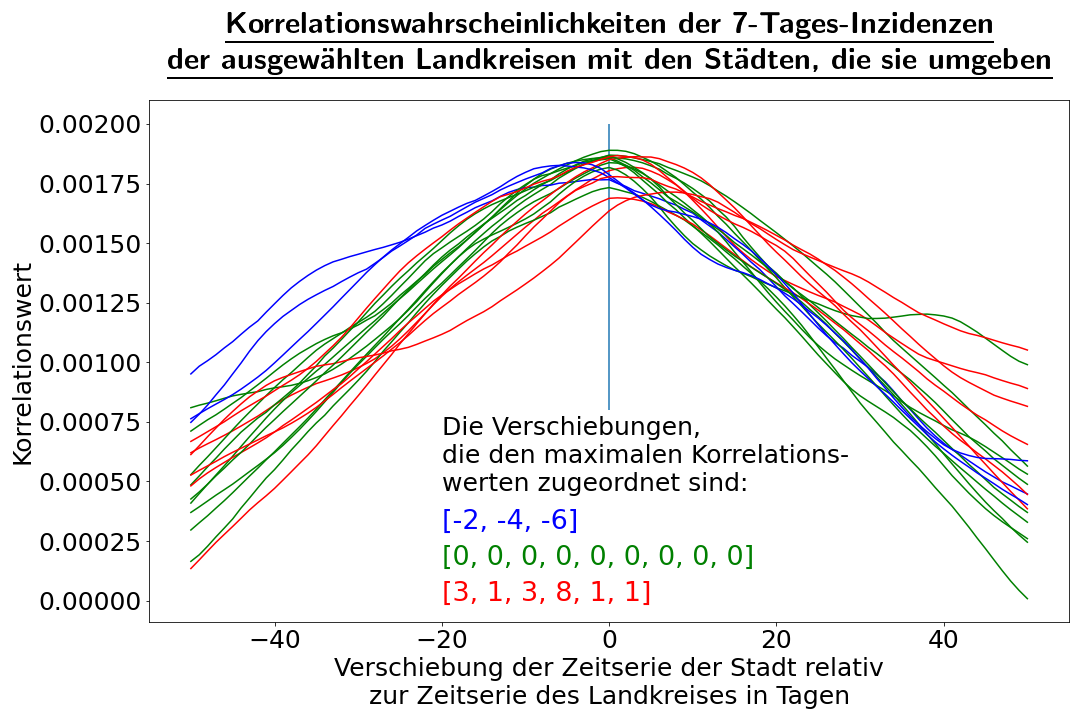
\includegraphics[width = 0.95\textwidth]{figures/Ergebnisse/highest_selected_counties.png}
    \caption{Die Korrelationswerte der 7-Tage-Inzidenzen der ausgewählten Landkreise mit den Städten, die sie umgeben. Die Kurven sind je nach dem x-Wert ihres Maximums eingefärbt: Orange bei positiven x-Werten, Blau bei negativen und grün bei einem x-Wert von null.}
    \label{fig:highest_selected_counties}
\end{figure}

In dieser sehr kleinen Teilmenge weisen 50~\% der Korrelationen den höchsten Korrelationswert bei einer Verschiebung von $\tau = 0$ auf.
Bei den Korrelationen aller deutschen Landkreise untereinander liegt bei 8.7~\% der höchste Korrelationswert bei einer Verschiebung von $\tau= 0$ (8.5~\% wenn man die Korrelationen der Landkreise mit sich selbst herausrechnet).

\autoref{fig:sum_selected_counties} zeigt die Tendenz der Verschiebung.
\begin{figure}
    \centering
    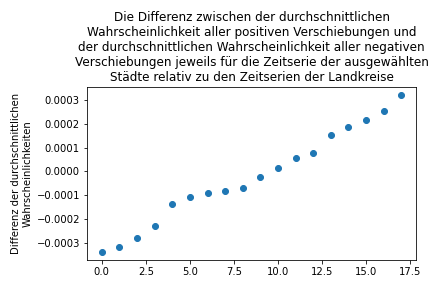
\includegraphics[width=0.95\textwidth]{figures/Ergebnisse/sum_selected_counties.png}
    \caption{Die Tendenzen der Verschiebung aus den Korrelationsanalysen der ausgewählten Städte und Landkreise.}
    \label{fig:sum_selected_counties}
\end{figure}